\chapter{Introduzione}

In molti problemi di interesse ingegneristico i fenomeni in esame presentano
direzioni preferenziali. Ad esempio in emodinamica \`e possibile incontrare problemi
simili dove la direzione del flusso \`e dominante rispetto alla dinamica
in direzione trasversale.
L'obbiettivo del progetto \`e l'implementazione in \texttt{LifeV} di un 
risolutore per un problema di diffusione trasporto reazione ( Advection Diffusion 
Reaction - ADR) 3D, basato sulla tecnica di Riduzione Gerarchica di Modello
(Hierarchical Model Reducation - HiMod).

HiMod si propone di sfruttare l'informazione
sulla presenza di una direzione dominante per ridurre il costo computazionale
della risoluzione convertendo un problema tridimensionale
in diversi problemi monodimensionali accoppiati.
La riduzione \`e resa possibile da uno sviluppo in serie di 
Fourier generalizzate della soluzione solo nella direzione trasversale. 
L'idea \`e quindi di approssimare soltanto i primi coefficienti di Fourier della soluzione.

\`E chiaro che il metodo non potr\`a essere competitivo rispetto al
metodo degli elementi finiti nel caso di problemi senza dinamiche dominanti,
tuttavia, dove la dinamica trasversale \`e semplice, consente di ottenere
una buona approssimazione del fenomeno, superiore rispetto a un modello
ridotto monodimensionale, ma senza i costi di una risoluzione 3D.

Approfondimenti riguardo alla Riduzione Gerarchica di Modello si possono trovare in
\cite{perotto:2008},\cite{perotto:2009},\cite{perotto:2012} e in \cite{zilio:himod} dove il metodo \`e stato 
applicato in un contesto bidimensionale (con condizioni di Dirichlet al bordo laterale) e parzialmente sviluppato dal punto di vista
teorico nel caso tridimensionale.

Nel progetto ci siamo focalizzati sull'implementazione del metodo in un contesto 
tridimensionale con una geometria semplice, ma con diverse tipologie di condizioni al bordo.
In particolare abbiamo implementato le basi istruite: una particolare scelta della base di Fourier
per la direzione trasversale in grade di incorporare le condizioni al bordo.


\section{Descrizione del metodo}

In questa sezione presenteremo le basi teoriche del metodo, applicandolo a un problema
di diffusione trasporto e reazione.

Consideriamo il seguente problema in un generico dominio $\Omega$, visto che il metodo 
\`e stato pensato soprattutto per applicazioni in emodinamica, consideriamo un dominio 
di forma tubolare
\begin{equation}
\label{eq: problema forte}
\begin{cases}
-\mu\Delta u + \vect{b}\cdot \nabla u + \sigma u = f & \text{in $\Omega$}\\
u=u_{in} & \text{su $\Gamma_{in}$}\\
\frac{\partial u}{\partial \vect{n}}=0 & \text{su $\Gamma_{out}$ }\\
u=0 & \text{su $\Gamma _{vaso}$} \\
\end{cases}
\end{equation}
\begin{center}
\begin{tikzpicture}
[scale=0.8]
\def\xi{0};
\def\xo{7};
\def\c{3.5};
\def\r{1};
\def\sig{2};
\def\rmax{0.5};
\def\rtot{\rmax+\r};

\draw[thick] (\xi,0) arc (90:270:0.3cm and \r cm);
\draw[dashed,thick] (\xi,-2*\r) arc (-90:90:0.3cm and \r cm);

\draw[thick] (\xo,0) arc (90:270:0.3cm and \r cm);
\draw[thick] (\xo,-2*\r) arc (-90:90:0.3cm and \r cm);

% \draw[->] (-2,0) -- (2,0);
% \draw[->] (0,-2) -- (0,2);
\draw[thick,parametric,domain=-\xi:\xo,samples=200,variable=\t] plot ({\t},{\rmax*exp{-pow(\t-\c,2)/\sig}});
\draw[thick,parametric,domain=-\xi:\xo,samples=200,variable=\t] plot ({\t},{-2*\r-\rmax*exp{-pow(\t-\c,2)/\sig}});
\draw[thick,parametric,domain=-\xi:\xo,samples=200,variable=\t,dashed] plot ({\t},{-\r});
\def\po{0.9};
\node[below] at (\xo*\po,-\r) {$\Omega_{1D}$};
\draw[pattern=north west lines, pattern color=gray, thick] (\c,-\r) ellipse (0.3 and \rtot);
\node[below] at (\c,-2*\r-\rmax) {$\gamma_x$};
\node[left] at(\xi-0.2,-\r) {$\Gamma_{in}$};
\node[right] at(\xo +0.2,-\r) {$\Gamma_{out}$};
\node at (\xi +0.5,-\r-0.7) {$\Omega$};
\node at (\c +2,-2*\r-0.4) {$\Gamma_{vaso}$};
\end{tikzpicture}
\end{center}
dove i coefficienti che compaiono nell'equazione sono tali per cui il problema variazionale associato 
sia ben posto in $V=H^1_{\Gamma_{IN}\cup\Gamma_{vaso}}(\Omega)$.
Immaginiamo di suddividere il dominio $\Omega$ in slice poste trasversalmente alla direzione longitudinale 
\begin{equation}
\label{eq:volume ridotto}
\Omega=\bigcup_{x\in \Omega_{1D}}\gamma_x.
\end{equation}
Ogni slice viene indicata con $\gamma_x$.
Lungo $\gamma_x$ vengono utilizzate funzioni spaziali differenti rispetto
a quelle utilizzate lungo $\Omega_{1D}$. 
Nel caso del tubo a sezione rettangolare, sul quale il codice si focalizzer\`a, $\Omega$ si riduce a $(0,L_x)\times\gamma$ 
dove $\gamma_x=\gamma=(0,L_y)\times(0,L_z)\quad\forall x\in(0,L_x)$
\begin{center}
\begin{tikzpicture}
[scale=1.5]

\draw [thick] (2,0) rectangle (3,1);
\node at (-0.25,1.25) {$\Gamma_{in}$};
\node at (3.3,0.5) {$\Gamma_{out}$};
\node at (2,1.75) {$\Gamma_{vaso}$};
\node at (0.5,0.4) {$\gamma$};
% \node at (0.7,0.88) {$\gamma}$};
\node at (3.5,-0.2) {$\Omega_{1D}$};


\draw [thick] (2,1)--(0,2)--(1,2)--(3,1);
\draw [thick] (2,0)--(0,1)--(0,2);

\draw [dashed,thick] (0,1)--(1,1)--(1,2);
\draw [dashed,thick] (1,1)--(3,0);

\draw [pattern=north west lines, pattern color=gray, thick] (0.5,0.75) rectangle (1.5,1.75);

\draw [thick,dashed, ->] (-0.5,2)--(3.5,0);

\end{tikzpicture}
\end{center}

Per gestire un dominio di forma generica \`e necessario utilizzare una mappa con la quale ricondursi ad un 
dominio di riferimento (si veda \cite{perotto:2008}. La teoria delle basi istruite, tuttavia, non \`e, ora, in grado di coprire 
il caso della mappa\footnote{In fase di implementazione abbiamo cominciato ad inserire le funzionalit\`a relative alla
mappa, ma ci siamo limitati ad aprire un branch sul repository (\texttt{20130710\_HiModMap})	 che, pur essendo praticamente 
completato, abbiamo dovuto abbandonare essendo incompatibile con le basi istruite. 
Con un altro tipo di base, ad esempio i polinomi di Legendre, \`e possibile recuperare il branch e 
completare l'implementazione.}.

Introduciamo alcuni spazi funzionali utili per ambientare correttamente il metodo.
Su $\Omega_{1D}$ utilizziamo lo spazio $V_{1D}=H^1_{\Gamma_{in}}(\Omega_{1D})$, 
mentre sulla fibra trasversale $\gamma$ introduciamo le basi modali $\left\{ \varphi_k \right\}_{k=1}^\infty$ 
ortonormali rispetto al prodotto scalare di $L^2(\gamma)$.
Quest'ultime definiscono su $\gamma$ lo spazio funzionale $V_{\gamma}:=span\left(\{\varphi_k\}_{k=1}^\infty\right)$.
\`E possibile dimostrare che, chiuso rispetto ad una opportuna norma, lo spazio $V_{1D}\otimes V_{\gamma}$ \`e isometricamente 
isomorfo a $V$. Per ulteriori dettagli sulla teoria e sulla notazione si pu\`o vedere la tesi di laurea di A. Zilio \cite{zilio:himod}.

Definiamo ora il sottospazio generato solo dai primi m modi ovvero  $V^m_{\gamma_x}:=span\{\varphi_1,...,\varphi_m\}$ e combiniamolo con $V_{1D}$, il risultato di tale operazione \`e il seguente spazio ridotto:
\begin{equation}
\label{spazio: ridotto}
V_m:=\left\{v_m(x,y,z)=\sum^m_{k=1}\varphi_k(y,z)\tilde{v}_k(x) ,\:\:con\:\:\tilde{v}_k\in V_{1D}\right\}.
\end{equation}

Questo \`e l'ambiente funzionale in cui opera HiMod.
L'ortogonalit\`a in $L^2(\gamma)$ implica che i coefficienti  $\tilde{v}_k$ che compaiono nella \eqref{spazio: ridotto} 
siano il risultato del seguente prodotto scalare
\begin{displaymath}
\tilde{v}_k(x)=\int_{\gamma}\varphi_k(y,z)v_m(x,y,z)\,dydz\quad\forall k=1\ldots m
\end{displaymath}
osserviamo come questi rappresentino, puntualmente, i coefficienti di Fourier della soluzione esatta rispetto alla base 
utilizzata sulla fibra trasversale.

La convergenza di una soluzione $u_m$ tale che soddisfi il problema \eqref{eq: problema forte}, nella sua forma variazionale
posta sul sottospazio $V_m$, discende dalle seguenti propriet\`a:
\begin{itemize}
\item[-] $V_m \subset V$ $\forall m\in \mathbb{N}$, ossia che lo spazio ridotto $V_m$ \`e \textbf{conforme} in $V$;
\item[-] $\displaystyle \lim_{m\to +\infty} \left(\inf_{v_m\in V_m}\mid\mid v-v_m\mid\mid\right)=0$ 
per ogni $v \in V$, ossia che vale la \textbf{propriet\`a di approssimazione} di $V_m$ rispetto a $V$;
\end{itemize}
Quest'approccio pu\`o essere esteso al caso di condizioni sulla parete laterale diverse dalle condizioni di Dirichlet omogenee.
In questo progetto abbiamo implementato l'approccio delle basi istruite, ma altre scelte sono possibili.

\section{Forma matriciale}
Per ogni $m\in\mathbb{N}$ consideriamo il seguente problema ridotto 

\noindent\emph{Trovare $u_m\in H^1(\Omega_{1D})\otimes V_{\gamma}^m$ tale che $\left.u_m\right|_{\Gamma_{in}}$ sia uguale alla proiezione del dato di Dirichlet 
su $V_\gamma^m$ e valga}
\begin{multline*}
\int_\Omega\left(\mu\nabla u_m\nabla v_m + \vect{b}\cdot\nabla u_mv_m+\sigma u_mv_m\right)\,d\Omega\quad \forall v_m\in V_m
=\int_\Omega fv \,d\Omega
\end{multline*}

Utilizziamo l'espansione di $u_m(x,y,z)$ 
rispetto alla base di Fourier 
\begin{equation}
\label{eq: espansione himod}
u_m(x,y,z)=\sum_{j=k}^m\tilde{u}_j(x)\varphi _j(y,z),\quad\tilde{u}_j(x)=\int_{\gamma}u_m(x,y,z) \varphi_j(y,z)\,dydz
\end{equation}
consideriamo inoltre funzioni test della forma 
$$v_m=\vartheta(x)\varphi _k(y,z),\quad \vartheta(x)\in V_{1D}\text{ e }
k=1,...m.$$ Il problema assume la seguente forma:

\begin{equation*}
\begin{split}
&\sum_{j=1}^m 
\int_\Omega\mu\nabla (\tilde{u}_j(x)\varphi _j(y,z))\nabla (\vartheta(x)\varphi _k(y,z))\,dxdydz\\
&+\int_\Omega(\vect{b}\nabla (\tilde{u}_j(x)\varphi _j(y,z))+\sigma\tilde{u}_j(x))\vartheta(x)\varphi _k(y,z)\,dxdydz\\
&=\int_\Omega f\vartheta(x)\varphi _k(y,z)\,dxdydz\\
\end{split}
\end{equation*}

Svolgendo l'operatore gradiente si ottiene:

\begin{equation*}
\begin{split}
&\sum_{j=1}^m
\int_\Omega\mu( \partial_x\tilde{u}_j \partial_x\vartheta\varphi _j\varphi _k + \tilde{u}_j \vartheta \partial_y\varphi _j\partial_y\varphi _k + \tilde{u}_j \vartheta \partial_z\varphi _j\partial_z\varphi _k)\,dxdydz \\
&+ \int_\Omega (b_1\partial_x\tilde{u}_j\varphi _j+b_2\tilde{u}_j\partial_y\varphi _j + b_3\tilde{u}_j\partial_z\varphi_j)\vartheta\varphi _k\,dxdydz\\ 
&+ \int_\Omega \sigma\tilde{u}_j\vartheta\varphi _j\varphi _k\,dxdydz \\
&=\int_\Omega f\vartheta\varphi _k\,dxdydz
\end{split}
\end{equation*}

Vediamo come il problema 2D si sia trasformato nella ricerca di $m$ funzioni monodimensionali.
Per semplicit\`a consideriamo una partizione $\tau_h$ uniforme lungo 
la fibra di supporto 1D.
Sia $N$ il numero di vertici lungo $\Omega_{1D}$.
Il passo della partizione \`e dunque $h=\vert \Omega_{1D}\vert / (N-1)$. 

Introduciamo lo spazio agli elementi finiti lungo $\Omega_{1D}$
\begin{equation*}
\label{eq: spazio polinomiale}
X_h^r= \left\{\psi_h \in C^0(\Omega_{1D}): \psi_h \vert_K  \in \mathbb{P}_r,\forall K\in T_h \right\}.
\end{equation*}
Per semplicit\`a supponiamo di utilizzare elementi finiti di grado uno, ma
la trattazione teorica \`e del tutto equivalente nel caso si volessero usare 
polinomi di grado pi\`u alto.
Una volta introdotta la discretizzazione lungo la direzione dominante 
del fenomeno \`e possibile esprimere i coefficienti di Fuorier 
nel seguente modo
\begin{equation*}
\label{eq: coeff fourier espansi}
\tilde{u}_j(x)=\sum_{s=1}^Nu_{js}\psi_s(x).
\end{equation*}
Abbiamo quindi discretizzato completamente il problema. Tramite l'espansione modale
siamo stati in grado di ridurre il problema da 3D a $m$ problemi 1D accoppiati che ora
abbiamo discretizzato con il metodo degli elementi finiti.

Otteniamo dunque la formulazione matriciale del problema\\
\emph{Trovare $\vect{u} \in \mathbb{R}^{N\cdot m}$ tale che}
\begin{equation*}
\begin{split}
&\sum_{j=1}^m \sum_{s=1}^N
u_{js} \Bigg[ \int_\Omega\mu( \partial_x\psi_s \partial_x\psi_l\varphi _j\varphi _k + \psi_s \psi_l \partial_y\varphi _j\partial_y\varphi _k + \psi_s \psi_l \partial_z\varphi _j\partial_z\varphi _k)\,dxdydz \\
&+ \int_\Omega (b_1\partial_x\psi_s\varphi _j+b_2\psi_s\partial_y\varphi _j + b_3\psi_s\partial_z\varphi_j)\psi_l\varphi _k\,dxdydz\\ 
&+\int_\Omega \sigma\psi_s\psi_l\varphi _j\varphi _k\,dxdydz \Bigg]\\
&=\int_\Omega f\psi_l\varphi _k\,dxdydz\quad \forall \psi_l\quad l=1\ldots N\quad\forall \varphi_k\quad k=1\ldots m
\end{split}
\end{equation*}
Per chiarezza abbiamo utilizzato un doppio indice $"js"$. Esso scorre in realt\`a  un vettore,
ma \`e possibile usare un solo indice che si lega a $"js"$ nel seguente modo
$$\vect{u}_{js}=\vect{u}[i]=\vect{u}[(j-1)N+s].$$ 
Integrando prima lungo la fibra trasversale si ottiene:

\begin{equation*}
\begin{split}
&\sum_{j=1}^m \sum_{s=1}^N
u_{js} \Bigg[ \int_{\Omega_{1D}}\mu\Bigg( \partial_x\psi_s \partial_x\psi_l\left(\int_{\gamma}\varphi _j\varphi _k\,dydz\right)\\
&+ \psi_s \psi_l \left(\int_{\gamma}\partial_y\varphi _j\partial_y\varphi _k\,dydz\right)
+ \psi_s \psi_l \left(\int_{\gamma}\partial_z\varphi _j\partial_z\varphi _k\,dydz\right)\Bigg)dx \\
&+ \int_{\Omega_{1D}}\Bigg( b_1\partial_x\psi_s\psi_l\left(\int_{\gamma}\varphi _j\varphi_k\,dydz\right)	
                    + b_2\psi_s          \psi_l\left(\int_{\gamma}\partial_y\varphi _j\varphi _k\,dydz\right)\\
&                    + b_3\psi_s          \psi_l\left(\int_{\gamma}\partial_z\varphi_j\varphi _k\,dydz\right)\Bigg)dx
+\int_{\Omega_{1D}} \sigma\psi_s\psi_l\left(\int_{\gamma}\varphi _j\varphi _k\,dydz\right)dx \Bigg]\\
&=\int_{\Omega_{1D}} f\psi_l\varphi _k\,dxdydz\quad \forall \psi_l\quad l=1\ldots N\quad\forall \varphi_k\quad k=1\ldots m.
\end{split}
\end{equation*}

Riordinando i termini

{\footnotesize
\begin{equation}
\begin{split}
\sum_{j=1}^m \sum_{s=1}^N\nsp{2}
u_{js}\nsp{1} \Bigg[\nsp{1}\int_{\Omega_{1D}}\nsp{4}&\underbrace{\left(\nsp{2}\int_{\gamma}\mu\varphi _j\varphi _k\,dydz\right)}_{Diffusione}
\partial_x\psi_s \partial_x\psi_l\\
+&\underbrace{\left(\nsp{2}\int_{\gamma}b_1\varphi _j\varphi_k\,dydz\right)}_{Trasporto}\partial_x\psi_s\psi_l\\
+&\underbrace{\Bigg(\nsp{2}\int_{\gamma}\mu\partial_y\varphi _j\partial_y\varphi _k
+ \mu\partial_z\varphi _j\partial_z\varphi _k
+ b_2\partial_y\varphi _j\varphi _k
+ b_3\partial_z\varphi_j\varphi _k
+ \sigma\varphi _j\varphi _k\,dydz\Bigg)}_{Reazione} \psi_s \psi_l dx \Bigg]\\
=\int_{\Omega_{1D}}\nsp{4}&\underbrace{\left(\nsp{2}\int_{\gamma}f\varphi _k\,dydz\right)}_{Forzante} \psi_ldx\quad \forall \psi_l\quad l=1\ldots N\quad\forall \varphi_k\quad k=1\ldots m. 
\end{split}
\end{equation}}

Da quest'ultima equazione \`e possibile riconoscere la struttura di un problema ADR 1D per ogni coppia $(j,k)$ con coefficienti che
comprimono le informazioni provenienti dalle direzioni trasversali.
Supponendo che i coefficienti siano costanti \`e possibile separare ulteriormente le variabili $(y,z)$. In questo modo
tutte le tre dimensioni fattorizzano con un enorme risparmio del tempo computazionale.

 La matrice generata ha dimensioni $(mN)^2$, tuttavia fissata
 la frequenza della soluziona e della funzione test, ossia fissando l'indice che scorre la base modale,
 \`e possibile identificare un blocco che corrisponde ad un problema monodimensionale.
Se utilizziamo gli elementi finiti di grado uno, il blocco \`e tridiagonale e
 la matrice ha un numero di elementi non zero pari a $m^2(3N-2)$. 
 Il pattern di sparsit\`a per un caso con m=3 e N=14 \`e riportato in figura \ref{fig:pattern}.
 \begin{figure}[!h]
    \centering
    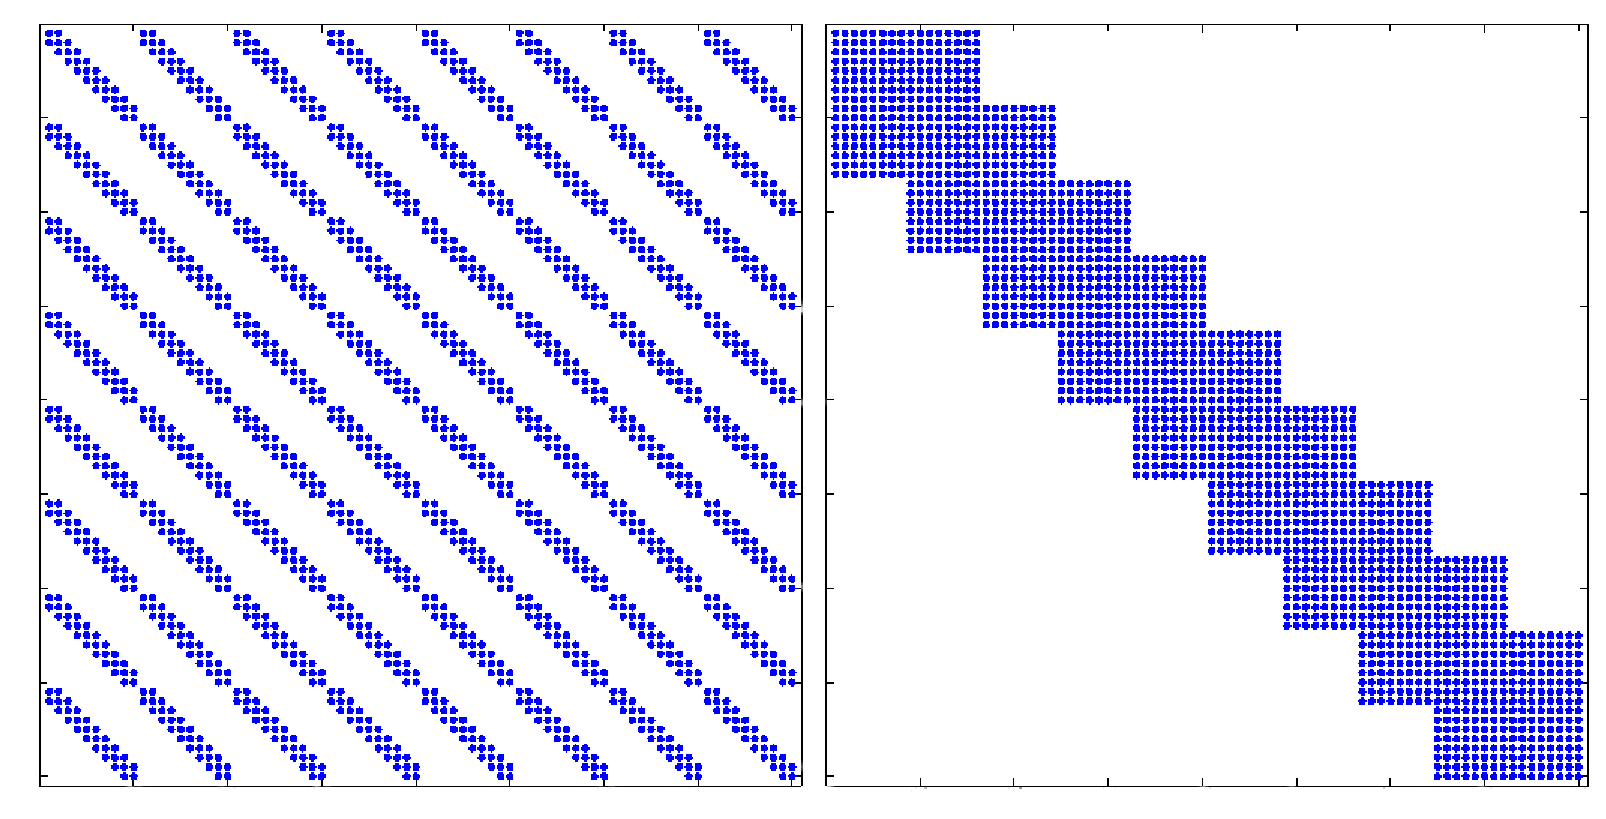
\includegraphics[scale = 0.45]{Varie/spy}
    \caption{Pattern di sparsit\`a per un caso con 9 elementi P1 e 8 modi.\\A sinistra il pattern che \`e stato poi utilizzato, a destra l'alternativa.}
    \label{fig:pattern}
\end{figure}
La matrice dei coefficienti \`e sparsa con un pattern noto a priori, ci\`o ha permesso 
 un assemblaggio pi\`u veloce in fase implementativa.
 \`E anche possibile riordinare la matrice in modo differente. Utilizzando una struttura 
 a blocchi associata ai gradi di libert\`a degli elementi finiti e non alla base modale.
 In questo modo avremmo una matrice tridiagonale a blocchi e ogni blocco sarebbe una matrice
 $m\times m$ piena. Con questa riordinamento della matrice la struttura \`e dunque quella 
 di un problema 1D dove invece che un solo grado di libert\`a associato al nodo ne sono associati $m$.
 Abbiamo implementato la prima scelta, che \`e quella suggerita in
 \cite{perotto:2008}, anche per poter sfruttare le procedure di assemblaggio 
 per gli elementi finiti 1D gi\`a presenti in LifeV.
\clearpage

\section{Basi istruite}
\label{sec: educated basis}
Le basi istruite sono state chiamate in questo modo perch\`e sono basi in grado di leggere la natura 
delle condizioni al bordo e di incorporarla all'interno della base stessa. Esse
conoscono parte del problema in esame.
Utilizzare le basi istruite equivale a imporre in maniera essenziale anche le condizioni al bordo 
naturali, come quelle di tipo Robin.
Il metodo delle basi istruite si basa sulla risoluzione di un problema agli autovalori 
ausiliario posto sulla fibra trasversale $\gamma$.\footnote{Nell'implementazione abbiamo risolto il
problema riportandolo sul quadrato di riferimento $(0,1)\times(0,1)$.} 
Introduciamo con un esempio l'algoritmo di costruzione delle basi istruite
\begin{itemize}
\item[\textbf{1.}] \textbf{Costruzione di un problema ausiliario} che rispecchi 
la natura delle condizioni alle pareti del problema originale (devono essere omogenee) e passaggio ai relativi problemi agli autovalori.
\mybox{
Nel caso si abbiano condizioni di Robin sull'intera parete del vaso, dovremo considerare il seguente problema ausiliario
\begin{equation}
\label{eq: problema RRRR}
\begin{cases}
-\Delta u(y,z)= 0 & \text{in $\gamma$}\\
\mu \nabla u(y,z) \cdot \vect{n} +\chi u(y,z)=0 & \text{su $\partial\gamma$}. \\
\end{cases}
\end{equation}
Si passi ora al problema agli autovalori associato al precedente sistema e 
ipotizzando la separazione di variabili $u(y,z)=\varphi(y)\vartheta(z)$, 
si arriva facilmente ai seguenti sottoproblemi agli autovalori
\begin{equation}
\label{eq: problema RR1}
\begin{cases}
-\varphi(y)'' = K_y\varphi(y) & \\
\mu \varphi(y)' +\chi \varphi(y) = 0 & \text{per $y=L_y$} \\
-\mu \varphi(y)'+\chi \varphi(y)=0 & \text{per $y=0$}. \\
\end{cases}
\end{equation}
\begin{equation}
\label{eq: problema RR2}
\begin{cases}
-\vartheta(z)'' = K_z\vartheta(z) & \\
\mu \vartheta(z)' +\chi \vartheta(z) = 0 & \text{per $z=L_z$} \\
-\mu \vartheta(z)'+\chi \vartheta(z)=0 & \text{per $z=0$} \\
\end{cases}
\end{equation}
}{Esempio - Robin BC}

\item[\textbf{2.}] \textbf{Identificazione del tipo di soluzione} dei problemi agli autovalori associati.

\mybox{
La generica soluzione dei sottoproblemi ottenuti \`e
\begin{equation}
\label{eq: 1sottoproblema}
\begin{array}{c}
\varphi (y)=A_ysin(\sqrt{K_y}y)+B_ycos(\sqrt{K_y}y) \\ \\
\vartheta (z)=A_zsin(\sqrt{K_z}z)+B_zcos(\sqrt{K_z}z).
\end{array}
\end{equation}

}{Esempio - Robin BC}

\item[\textbf{3.}] \textbf{Ricerca degli autovalori di un sottoproblema} tramite risoluzione dell'equazione non lineare associata ad esso, ottenuta risolvendo le condizioni di bordo.
\mybox{
Nel caso trattato in esempio le equazioni che si ottengono sono le seguenti ($x = \sqrt{K_y}$ e $w= \sqrt{K_z}$)
\begin{equation}
\label{eq: funzione autovalori}
\begin{array}{c}
f(x)= 2\mu x + tan(L_y x)\left(\chi - \frac{\mu ^2 x^2 }{\chi} \right) \\ \\
f(w)= 2\mu w + tan(L_z w)\left(\chi - \frac{\mu ^2 w^2 }{\chi} \right).
\end{array}
\end{equation}
}{Esempio - Robin BC}
\end{itemize}
Per giustificare l'algoritmo dal punto di vista teorico riportiamo solamente un teorema
che analizza un generico problema agli autovalori. Per adattarlo al nostro caso
\`e sufficiente scegliere $H=L^2(\gamma)$ e $V=H^1_{\partial\gamma_o}(\gamma)$, dove $\partial\gamma_0$ \`e il sottoinsieme
di $\partial\gamma$ dove sono imposte le condizioni di Dirichlet e la forma bilineare $a$ si riferisce alla forma variazionale
associata al problema ausiliario agli autovalori, per ulteriori dettagli si veda \cite{salsa2004equazioni}.
\begin{teorema}
\label{teo: salsa}
Siano V,H spazi di Hilbert, con H separabile, V denso in H, e tali che
l'immersione di V in H sia compatta. Sia a( , ) una forma bilineare in V,
continua, simmetrica e debolmente coerciva. 
Allora
\begin{description}
\item[(a)] $\sigma(a)=\sigma_p(a)\subset(-\lambda_0,+\infty)$. Inoltre, se la successione degli autovalori $\{\lambda_m \}_{m\geq 1}$ \`e infinita allora $\lambda_m\rightarrow +\infty$;
\item[(b)] se u ,v sono autovettori corrispondenti ad autovalori differenti, allora a(u,v) = 0 = (u,v). Inoltre, H ha una base ortonormale $\{ u_m \}_{m\geq 1}$ di autovettori di a;
\item[(c)] la successione $\{u_m / \sqrt{\lambda_0+\lambda_m} \}_{m\geq 1}$ costituisce una base ortonormale in V, rispetto al prodotto scalare
\begin{displaymath}
((u,v))=a(u,v)+\lambda_0 (u,v).
\end{displaymath}
\end{description}
\end{teorema}
$\sigma$ \`e lo spettro della forma bilineare $a$, $\sigma_p$ il suo spettro puntuale, $\lambda_0$ \`e l'eventuale costante necessaria per la debole coercivit\`a.
La base che si ottiene \`e dunque ortonormale rispetto al prodotto scalare $L^2(\gamma)$.

\mybox{
Nel caso di condizioni al bordo di Dirichlet il problema si semplifica. 
Infatti non occorre risolvere l'equazione non-lineare:	
gli autovalori che si ottengono sono noti a priori e sono della forma
\begin{equation}
\label{eq: problema agli autovalori dirichlet}
\begin{array}{c l}
K_{y,p} = \left( \frac{\pi p}{L_y}\right)^2 & p = 1, ... ,m_y\\
K_{z,q} = \left( \frac{\pi q}{L_z}\right)^2 & q = 1, ... ,m_z\\
\lambda_{p,q}=K_{y,p}+K_{z,q}.&\\
\end{array}
\end{equation}
}{Osservazione -- Caso condizioni al bordo di Dirichlet}
Numericamente, o analiticamente come nel caso di condizioni al bordo di Dirichlet, \`e possibile
trovare gli autovalori dei sottoproblemi monodimensionali. La difficolt\`a
st\`a nel legarli in modo opportuno agli autovalori del problema bidimensionale in modo che 
venga preservato l'ordinamento crescente degli autovalori 2D rispetto all'indice $k$ della base modale.
In particolare \`e necessario costruire una mappa che leghi ad ogni frequenza $k$ 
la corretta coppia $(p,q)$, per farlo abbiamo sviluppato un algoritmo che verr\`a descritto 
nel capitolo relativo all'implementazione.
\clearpage